\documentclass[12pt,twoside,a4paper]{report}
\usepackage[a4paper,width=150mm,top=25mm,bottom=25mm,bindingoffset=6mm]{geometry}

\usepackage[utf8x]{inputenc}
\usepackage[slovak]{babel}
\usepackage{palatino,verbatim}

% Balicek pre priamu rec - \say
\usepackage{dirtytalk}

% Balicek "alltt" je to iste ako "verbatim" mod, ale navyse podporuje aj formatovacie znacky textu
\usepackage{alltt}

% Obrazky
\usepackage{graphicx}
\graphicspath{ {obr/} }

% Cislovanie obrazkov a tabuliek
\usepackage{chngcntr}
%Cisluj obrazky nezavisle od cisla kapitol/podkapitol
\counterwithout{figure}{subsection}
\counterwithout{table}{subsection}

% Referencovanie kapitol/sekcii/... podľa ich nadpisu
\usepackage{nameref}

% Tabulky s viacriadkovymi bunkami a zlucenymi bunkami
% Tabulky generujem naastrojom "http://www.tablesgenerator.com/"
\usepackage{booktabs}
\usepackage{multirow}
% LaTeX ma problemy s prikazmi cline a cmidrule, ked je babel nastaveny na slovencinu/cestinu, kvoli definicii pomlcky
% NAMIESTO POMLCKY POUZI ZNAK ZNAMIENKA MINUS "−" (plati hlavne v nazvoch nadpisov a labelov)
\usepackage{etoolbox}
\preto\tabular{\shorthandoff{-}}

%Uloz obrazok tam, kde je deklarovany
%\usepackage[subsection]{placeins}

% Pisanie v slovenčine
\newcommand\sktxt[1]{\foreignlanguage{slovak}{#1}}

% Tabulator
\newcommand\tab[1][1cm]{\hspace*{#1}}

\begin{document}
\pagenumbering{arabic}

\setcounter{chapter}{1}
\chapter*{MPLS}
\paragraph{}
Andrej Šišila, Marián Vachalík

\tableofcontents

\newpage
\section{Topológia}
\paragraph{}
Budeme konfigurovať smerovacie protokoly MPLS a IS-IS na topológií, ktorá je znázornená na obrázku \ref{fig:mpls_isis_topo}. V rámci autonómnych systémov sme konfigurovali smerovacie protokoly IS-IS (pokiaľ má autonómny systém viac ako 2 smerovače) a BGP (iBGP). Medzi autonómnymi systémami sme konfigurovali len BGP (eBGP). IP adresácia je uvedená v tabuľke \ref{tab:ip_adresacia} a dopĺňa grafické znázornenie topológie na obrázku \ref{fig:mpls_isis_topo}. Smerovače R6 a R7 sme nekonfigurovali.

\begin{figure}[!htbp]
\centering
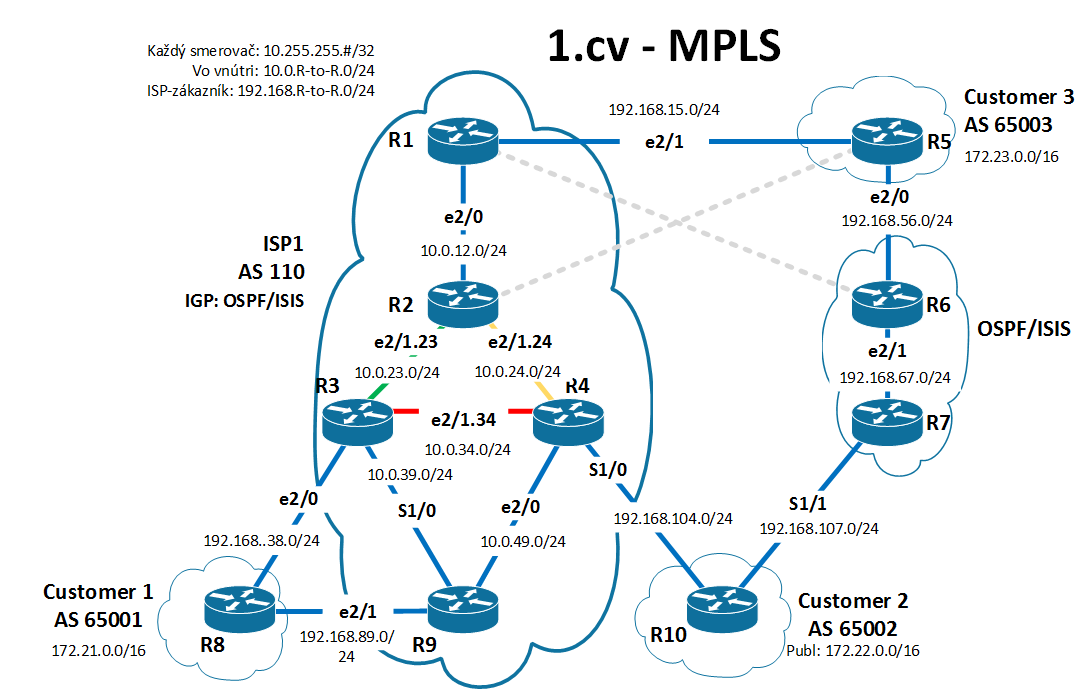
\includegraphics[width=14cm,keepaspectratio]{mpls_isis_topo}
\caption{Topológia MPLS + L3VPN}
\label{fig:mpls_isis_topo}
\end{figure}



\clearpage


\begin{table}[!htbp]
\centering
\caption{IP adresácia}
\label{tab:ip_adresacia}
\begin{tabular}{|c|l|l|l|}
\hline
\textbf{Smerovač}    & \multicolumn{1}{c|}{\textbf{Rozhranie}} & \multicolumn{1}{c|}{\textbf{IP adresa}} & \multicolumn{1}{c|}{\textbf{Maska}} \\ \hline
\multirow{3}{*}{R1}  & E2/0                                    & 10.0.12.1                               & 255.255.255.0                       \\ \cline{2-4} 
                     & E2/1                                    & 192.168.15.1                            & 255.255.255.0                       \\ \cline{2-4} 
                     & Lo0                                     & 10.255.255.1                            & 255.255.255.255                     \\ \hline
\multirow{4}{*}{R2}  & E2/0                                    & 10.0.12.2                               & 255.255.255.0                       \\ \cline{2-4} 
                     & E2/1.23                                 & 10.0.23.2                               & 255.255.255.0                       \\ \cline{2-4} 
                     & E2/1.24                                 & 10.0.24.2                               & 255.255.255.0                       \\ \cline{2-4} 
                     & Lo0                                     & 10.255.255.2                            & 255.255.255.255                     \\ \hline
\multirow{4}{*}{R3}  & E2/0                                    & 192.168.38.3                            & 255.255.255.0                       \\ \cline{2-4} 
                     & E2/1.23                                 & 10.0.23.3                               & 255.255.255.0                       \\ \cline{2-4} 
                     & E2/1.34                                 & 10.0.34.3                               & 255.255.255.0                       \\ \cline{2-4} 
                     & Lo0                                     & 10.255.255.3                            & 255.255.255.255                     \\ \hline
\multirow{5}{*}{R4}  & S1/0                                    & 192.168.104.4                           & 255.255.255.0                       \\ \cline{2-4} 
                     & E2/0                                    & 10.0.49.4                               & 255.255.255.0                       \\ \cline{2-4} 
                     & E2/1.24                                 & 10.0.24.4                               & 255.255.255.0                       \\ \cline{2-4} 
                     & E2/1.34                                 & 10.0.34.4                               & 255.255.255.0                       \\ \cline{2-4} 
                     & Lo0                                     & 10.255.255.4                            & 255.255.255.255                     \\ \hline
\multirow{4}{*}{R5}  & E2/0                                    & 192.168.56.5                            & 255.255.255.0                       \\ \cline{2-4} 
                     & E2/1                                    & 192.168.15.5                            & 255.255.255.0                       \\ \cline{2-4} 
                     & Lo0                                     & 10.255.255.5                            & 255.255.255.255                     \\ \cline{2-4} 
                     & Lo1                                     & 172.23.0.1                              & 255.255.0.0                         \\ \hline
\multirow{3}{*}{R6}  & E2/0                                    & 192.168.56.6                            & 255.255.255.0                       \\ \cline{2-4} 
                     & E2/1                                    & 192.168.67.6                            & 255.255.255.0                       \\ \cline{2-4} 
                     & Lo0                                     & 10.255.255.6                            & 255.255.255.255                     \\ \hline
\multirow{3}{*}{R7}  & E2/1                                    & 192.168.67.7                            & 255.255.255.0                       \\ \cline{2-4} 
                     & S1/1                                    & 192.168.107.7                           & 255.255.255.0                       \\ \cline{2-4} 
                     & Lo0                                     & 10.255.255.7                            & 255.255.255.255                     \\ \hline
\multirow{4}{*}{R8}  & E2/0                                    & 192.168.38.8                            & 255.255.255.0                       \\ \cline{2-4} 
                     & E2/1                                    & 192.168.89.8                            & 255.255.255.0                       \\ \cline{2-4} 
                     & Lo0                                     & 10.255.255.8                            & 255.255.255.0                       \\ \cline{2-4} 
                     & Lo1                                     & 172.21.0.1                              & 255.255.0.0                         \\ \hline
\multirow{4}{*}{R9}  & E2/0                                    & 10.0.49.9                               & 255.255.255.0                       \\ \cline{2-4} 
                     & E2/1                                    & 192.168.89.9                            & 255.255.255.0                       \\ \cline{2-4} 
                     & Lo0                                     & 10.255.255.9                            & 255.255.255.255                     \\ \cline{2-4} 
                     & Lo1                                     & 172.21.0.1                              & 255.255.0.0                         \\ \hline
\multirow{4}{*}{R10} & S1/0                                    & 192.168.104.10                          & 255.255.255.0                       \\ \cline{2-4} 
                     & S1/1                                    & 192.168.107.10                          & 255.255.255.0                       \\ \cline{2-4} 
                     & Lo0                                     & 10.255.255.10                           & 255.255.255.255                     \\ \cline{2-4} 
                     & Lo1                                     & 172.22.0.1                              & 255.255.0.0                         \\ \hline
\end{tabular}
\end{table}


% Novu kapitolu davam na novu stranu, lebo bez toho mi zobrazuje tabulku v dalsej kapitole, kde ale tabulka nepatri.
\clearpage

\section{Úlohy}
\subsection{IS−IS alebo OSPF}
\subsubsection{Popis}
\paragraph{}
Ako vnútorný smerovací protokol sme zvolili IS-IS. Jeho konfigurácia je rovnaká ako v predchádzajúcich cvičeniach s ohľadom na aktuálny adresný plán.

\subsubsection{Konfigurácia}
\paragraph{}
IS-IS sme konfigurovali na R1, R2, R3, R4 a R9

\noindent
{\fontfamily{qcr}\selectfont
\begin{small}
\begin{alltt}
R1(config)#router isis
  net 49.0002.0102.5525.5001.00
  exit
int e2/0
  ip router isis
  isis network point-to-point
int lo0
  ip router isis
\end{alltt}
\end{small}
}

\subsubsection{Overenie}
\paragraph{}
Konfiguráciu IS-IS sme overovali zobrazením IS-IS databázy. Nižšie uvádzame výpis príkazu \say{show isis database} zo smerovača R1.

\noindent
{\fontfamily{qcr}\selectfont
\begin{small}
\begin{alltt}
R1#sh isis database 

Tag null:
IS-IS Level-1 Link State Database:
LSPID                 LSP Seq Num  LSP Checksum  LSP Holdtime      ATT/P/OL
R1.00-00            * 0x000004BE   0x23C9        944               0/0/0
R2.00-00              0x000004BD   0x5254        619               0/0/0
R3.00-00              0x000004C3   0x3539        945               0/0/0
R3.01-00              0x000004BE   0x0B18        733               0/0/0
R4.00-00              0x000004C2   0x4758        420               0/0/0
R4.01-00              0x000004BB   0x170D        465               0/0/0
R4.02-00              0x000004BC   0x27F9        900               0/0/0
R9.00-00              0x000004C0   0x0BD0        1084              0/0/0
IS-IS Level-2 Link State Database:
LSPID                 LSP Seq Num  LSP Checksum  LSP Holdtime      ATT/P/OL
R1.00-00            * 0x000004C6   0x7857        787               0/0/0
R2.00-00              0x000004C1   0x9FB1        1186              0/0/0
R3.00-00              0x000004C8   0xE562        973               0/0/0
R3.01-00              0x000004BE   0x9A11        1157              0/0/0
R4.00-00              0x000004CB   0x89ED        973               0/0/0
R4.01-00              0x000004BE   0xA009        1146              0/0/0
R4.02-00              0x000004B6   0xC2EC        1122              0/0/0
R9.00-00              0x000004C2   0xAE2A        768               0/0/0
\end{alltt}
\end{small}
}


\paragraph{}
Z výpisu vyplýva, že protokol IS-IS na R1 je spustený. IS-IS databáza na R1 obsahuje aj záznamy o smerovačoch, ktoré sa nacáhádzajú v oblasti 110 t.j. R2, R3, R4 a R9. Z toho vyplýva, že IS-IS je spustený v celej oblasti 110.











\subsection{MPLS}
\subsubsection{Popis}
\paragraph{}
Základnú konfiguráciu MPLS sme vypracovali podľa stránky \say{nil.uniza.sk}. Najprv zapneme \say{Cisco express forwarding} príkazom \say{ip cef}. Nakoniec zapneme MPLS príkazom \say{mpls ip}. Príkaz \say{mpls ip} sme použili iba na rozhraniach vnútri providerskej siete, nie na PE smerovačoch smerom k zákazníkom.

\subsubsection{Konfigurácia}
\paragraph{}
Aby sme zabezpečili konektivitu medzi jednotlivými zákazníkmi R5, R8 a R10, je potrebné nakonfigurovať BGP medzi týmito smerovačmi a ich susedmi v ISP1. Rovnako aj ohlasujeme požadovanú sieť zákazníka, v našom prípade Lo0. Na smerovači R2 BGP nekonfigurujeme.

\noindent
{\fontfamily{qcr}\selectfont
\begin{small}
\begin{alltt}
R1 (config)#ip cef
mpls ip
int serial1/0
  mpls ip
router bgp 65001
  neighbor 192.168.15.1 remote-as 110
  address-family ipv4 unicast
  neighbor 192.168.15.1 activate
  network 10.255.255.5 mask 255.255.255.255
\end{alltt}
\end{small}
}

\subsubsection{Overenie}
\paragraph{}
\noindent
{\fontfamily{qcr}\selectfont
\begin{small}
\begin{alltt}
R10#sh ip bgp ipv4 unicast
...

     Network          Next Hop            Metric LocPrf Weight Path
 *>  10.255.255.5/32  192.168.104.4                          0 110 110 i
 *>  10.255.255.8/32  192.168.104.4                          0 110 110 i
 *>  10.255.255.10/32 0.0.0.0                  0         32768 i
 *>  \textbf{172.21.0.0}       192.168.104.4                          0 110 110 ?
 *>  \textbf{172.22.0.0}       0.0.0.0                  0         32768 ?
 *>  \textbf{172.23.0.0}       192.168.104.4                          0 110 110 ?
...




R10#traceroute 10.255.255.8 source l0
Type escape sequence to abort.
Tracing the route to 10.255.255.8
VRF info: (vrf in name/id, vrf out name/id)
  1 192.168.104.4 24 msec 16 msec 16 msec
  2 192.168.38.3 [AS 110] \textbf{[MPLS: Label 26 Exp 0]} 16 msec 36 msec 36 msec
  3 192.168.38.8 [AS 110] 68 msec *  52 msec
R10#

\end{alltt}
\end{small}
}

\paragraph{}
Z výpisu \say{show ip bgp ipv4 unicast} z klientského smerovača R10 vyplýva, že vidíme zákaznícke siete aj zo smerovačov R5 a R8. Na výpise \say{traceroute 10.255.255.8 source l0} vidíme, že paketu bola priradená MPLS značka.




\subsection{LDP alebo RSVP}
\subsubsection{Popis}
\paragraph{}
Dohodli sme sa, že aktivujeme LDP (Label Distribution Protocol), aby si smerovače mohli MPLS značky posielať medzi sebou.

\subsubsection{Konfigurácia}
\paragraph{}
Na kažom providerskom smerovači sme v globálnom konfiguračnom režime aktivovali LDP príkazom:

\noindent
{\fontfamily{qcr}\selectfont
\begin{small}
\begin{alltt}
mpls label protocol ldp
\end{alltt}
\end{small}
}

\subsubsection{Overenie}
\paragraph{}
Funkčnosť LDP sme overovali príkazom \say{show mpls ldp discovery} na providerských smerovačoch. Nižšie je uvedený výpis z R3.

\noindent
{\fontfamily{qcr}\selectfont
\begin{small}
\begin{alltt}
R3#show mpls ldp discovery
 Local LDP Identifier:
    10.255.255.3:0
    Discovery Sources:
    Interfaces:
	Serial1/0 (ldp): xmit/recv
	    LDP Id: 10.255.255.9:0
	Ethernet2/1.23 (ldp): xmit/recv
	    LDP Id: 10.255.255.2:0
	Ethernet2/1.34 (ldp): xmit/recv
	    LDP Id: 10.255.255.4:
\end{alltt}
\end{small}
}

\paragraph{}
Z výpisu vyplýva, že R3 vidí aktívne LDP na susedných providerských smerovačoch R2, R4 a R9.














\subsection{Router Reflector alebo konfederácie}
\subsubsection{Popis}
\paragraph{}
V tomto prípade sme sa dohodli o nastavení Route Reflectora (RR) na smerovač R1. RR je BGP smerovač, ktorý obchádza pravidlo, že iBGP topológia musí byť \say{full-mesh} t.j. iBGP smerovač v jednej oblasti nešíri prefixy, ktoré sa naučil cez iBGP smerovač z inej oblasti.



\subsubsection{Konfigurácia}
\paragraph{}
Smerovače R3, R4 a R9 sme nakonfigurovali tak, aby používali R1 ako RR.

\noindent
{\fontfamily{qcr}\selectfont
\begin{small}
\begin{alltt}
!R3, R4, R9
router bgp 110
  neighbor 10.255.255.1 remote-as 110
  neighbor 10.255.255.1 update-source Loopback0
  address-family ipv4 unicast
    neighbor 10.255.255.1 activate
    neighbor 10.255.255.1 next-hop-self
  network 10.255.255.3 mask 255.255.255.255
\end{alltt}
\end{small}
}

\paragraph{}
Potom sme nakonfigurovali R1 ako RR.

\noindent
{\fontfamily{qcr}\selectfont
\begin{small}
\begin{alltt}
!R1
router bgp 110
  neighbor 10.255.255.3 remote-as 110
  neighbor 10.255.255.3 update-source l0
  neighbor 10.255.255.4 remote-as 110
  neighbor 10.255.255.4 update-source l0
  neighbor 10.255.255.9 remote-as 110
  neighbor 10.255.255.9 update-source l0
  address-family ipv4 unicast
    neighbor 10.255.255.3 route-reflector-client
    neighbor 10.255.255.3 send-community extended
    neighbor 10.255.255.3 next-hop-self
    neighbor 10.255.255.3 activate
    neighbor 10.255.255.4 route-reflector-client
    neighbor 10.255.255.4 send-community extended
    neighbor 10.255.255.4 next-hop-self
    neighbor 10.255.255.4 activate
    neighbor 10.255.255.9 route-reflector-client
    neighbor 10.255.255.9 send-community extended
    neighbor 10.255.255.9 next-hop-self
    neighbor 10.255.255.9 activate 
\end{alltt}
\end{small}
}

\subsubsection{Overenie}
\paragraph{}
Konektivita by mala byť v tomto prípade už všade. Presvedčíme sa pomocou tcl skriptu.

\noindent
{\fontfamily{qcr}\selectfont
\begin{small}
\begin{alltt}
R1#tclsh
R1(tcl)#foreach address {
+>(tcl)#10.255.255.1
+>(tcl)#10.255.255.2
+>(tcl)#10.255.255.3
+>(tcl)#10.255.255.4
+>(tcl)#10.255.255.5
+>(tcl)#10.255.255.6
+>(tcl)#10.255.255.7
+>(tcl)#10.255.255.8
+>(tcl)#10.255.255.9
+>(tcl)#10.255.255.10
+>(tcl)#} {
+>(tcl)#ping $address source 10.255.255.1}
Sending 5, 100-byte ICMP Echos to 10.255.255.1, timeout is 2 seconds:
!!!!!
Success rate is 100 percent (5/5), round-trip min/avg/max = 8/8/8 ms
Sending 5, 100-byte ICMP Echos to 10.255.255.2, timeout is 2 seconds:
!!!!!
Success rate is 100 percent (5/5), round-trip min/avg/max = 16/22/28 ms
Sending 5, 100-byte ICMP Echos to 10.255.255.3, timeout is 2 seconds:
!!!!!
Success rate is 100 percent (5/5), round-trip min/avg/max = 24/39/68 ms
Sending 5, 100-byte ICMP Echos to 10.255.255.4, timeout is 2 seconds:
!!!!!
Success rate is 100 percent (5/5), round-trip min/avg/max = 16/33/52 ms
Sending 5, 100-byte ICMP Echos to 10.255.255.5, timeout is 2 seconds:
!!!!!
Success rate is 100 percent (5/5), round-trip min/avg/max = 16/26/40 ms
Sending 5, 100-byte ICMP Echos to 10.255.255.8, timeout is 2 seconds:
!!!!!
Success rate is 100 percent (5/5), round-trip min/avg/max = 72/88/100 ms
Sending 5, 100-byte ICMP Echos to 10.255.255.9, timeout is 2 seconds:
!!!!!
Success rate is 100 percent (5/5), round-trip min/avg/max = 48/63/80 ms
Sending 5, 100-byte ICMP Echos to 10.255.255.10, timeout is 2 seconds:
!!!!!
Success rate is 100 percent (5/5), round-trip min/avg/max = 72/79/100 ms





R4#ping vrf GREEN 172.21.0.1
Type escape sequence to abort.
Sending 5, 100-byte ICMP Echos to 172.21.0.1, timeout is 2 seconds:
!!!!!
Success rate is 100 percent (5/5), round-trip min/avg/max = 20/31/40 ms
R4#ping vrf GREEN 172.22.0.1
Type escape sequence to abort.
Sending 5, 100-byte ICMP Echos to 172.22.0.1, timeout is 2 seconds:
!!!!!
Success rate is 100 percent (5/5), round-trip min/avg/max = 12/23/36 ms
R4#ping vrf GREEN 172.23.0.1
Type escape sequence to abort.
Sending 5, 100-byte ICMP Echos to 172.23.0.1, timeout is 2 seconds:
!!!!!
Success rate is 100 percent (5/5), round-trip min/avg/max = 44/56/72 ms
\end{alltt}
\end{small}
}

\paragraph{}
Z výpisov z R1 vyplýva, že konektivita zostala zachovaná ku všetkým smerovačom v oblasti 110. S použitím VRF pingu z R4 sme zistili, že aj zákaznícke siete sú stále dostupné.










\subsection{Multiprotocol BGP}
\subsubsection{Popis}
\paragraph{}
Multiprotokolové BGP (MP-BGP) je kombinácia BGP s, v tomto prípade, MPLS. Tak možeme poskytovať L3VPN službu viacerým zákazníkom, v tomto prípade zákazníkom RED a GREEN.

\paragraph{}
Zákazník RED mal loopback0 rozhrania s IP adresami 172.[21/22/23].0.1 /16 v AS 65001, 65002 a 65003. Zákazník GREEN mal dve loopback1 rozhrania: jedno na R1, druhé na R9 s IP adresami 172.[21/22].0.1 /16.

\subsubsection{Konfigurácia}
\paragraph{}
MP-BGP sme konfigurovali na všetkých PE smerovačoch t.j. R1, R3, R4 a R9. Nižšie je uvedená konfigurácia pre R1.

\noindent
{\fontfamily{qcr}\selectfont
\begin{small}
\begin{alltt}
R1(config)#ip cef
mpls label protocol ldp

ip vrf GREEN
 rd 100:2 
 route-target export 110:2
 route-target import 110:2
 exit
ip vrf RED
 rd 110:1
 route-target export 110:1
 route-target import 110:1
 exit

interface Loopback0
 ip address 10.255.255.1 255.255.255.255
 ip router isis

interface Loopback1
 ip address 172.21.0.1 255.255.0.0
 ip vrf forwarding GREEN

interface Ethernet2/0
 ip address 10.0.12.1 255.255.255.0
 ip router isis 
 duplex half
 mpls ip
 isis network point-to-point 

interface Ethernet2/1
 ip vrf forwarding RED
 ip address 192.168.15.1 255.255.255.0
 duplex half

router bgp 110
 bgp log-neighbor-changes
 neighbor 10.255.255.3 remote-as 110
 neighbor 10.255.255.3 update-source Loopback0
 neighbor 10.255.255.4 remote-as 110
 neighbor 10.255.255.4 update-source Loopback0
 neighbor 10.255.255.9 remote-as 110
 neighbor 10.255.255.9 update-source Loopback0

 address-family vpnv4
  neighbor 10.255.255.3 activate
  neighbor 10.255.255.3 send-community extended
  neighbor 10.255.255.3 route-reflector-client
  neighbor 10.255.255.4 activate
  neighbor 10.255.255.4 send-community extended
  neighbor 10.255.255.4 route-reflector-client
  neighbor 10.255.255.9 activate
  neighbor 10.255.255.9 send-community extended
  neighbor 10.255.255.9 route-reflector-client
 exit-address-family
 
 address-family ipv4 vrf GREEN
  redistribute connected
 exit-address-family
 
 address-family ipv4 vrf RED
  redistribute connected
  neighbor 192.168.15.5 remote-as 65001
  neighbor 192.168.15.5 activate
  neighbor 192.168.15.5 as-override
 exit-address-family
\end{alltt}
\end{small}
}


\subsubsection{Overenie}
\paragraph{}
Funkčnosť BGP sme overovali príkazmi \say{show ip bgp vpnv4 vrf RED}, \say{show ip bgp vpnv4 vrf GREEN} a \say{show ip bgp vpnv4 vrf RED 172.21.0.0} na PE smerovačoch a príkazom \say{show ip bgp} na Customer Edge (CE) smerovačoch.

\noindent
{\fontfamily{qcr}\selectfont
\begin{small}
\begin{alltt}
R1#show ip bgp vpnv4 vrf RED
BGP table version is 144, local router ID is 10.255.255.1
...

     Network          Next Hop            Metric LocPrf Weight Path
Route Distinguisher: 110:2 (default for vrf RED)
 * i 172.21.0.0       10.255.255.9             0    100      0 65001 ?
 *>i                  10.255.255.3             0    100      0 65001 ?
 *>i 172.22.0.0       10.255.255.4             0    100      0 65002 ?
 *>  172.23.0.0       192.168.15.5             0             0 65003 ?
...





R1#show ip bgp vpnv4 vrf GREEN
BGP table version is 144, local router ID is 10.255.255.1
...

     Network          Next Hop            Metric LocPrf Weight Path
Route Distinguisher: 110:2 (default for vrf RED)
 * i 172.21.0.0       0.0.0.0                  0    100      0 65004 ?
 *>i 172.22.0.0       10.255.255.9             0    100      0 65005 ?
...




R8#show ip bgp
BGP table version is 47, local router ID is 10.255.255.8
...

     Network          Next Hop            Metric LocPrf Weight Path
...
 *>  172.21.0.0       0.0.0.0                  0         32768 ?
 *   172.22.0.0       192.168.89.9                           0 110 110 ?
 *>                   192.168.38.3                           0 110 110 ?
 *   172.23.0.0       192.168.89.9                           0 110 110 ?
 *>                   192.168.38.3                           0 110 110 ?
...




R1#show ip bgp vpnv4 vrf RED 172.21.0.0
BGP routing table entry for 110:2:172.21.0.0/16, version 142
Paths: (2 available, best #2, table RED)
  Advertised to update-groups:
     9          3         
  Refresh Epoch 10
  65001, (Received from a RR-client)
    10.255.255.9 (metric 40) from 10.255.255.9 (10.255.255.9)
      Origin incomplete, metric 0, localpref 100, valid, internal
      Extended Community: RT:110:2
      Connector Attribute: count=1
       type 1 len 12 value 110:2:10.255.255.9
      mpls labels in/out nolabel/24
      rx pathid: 0, tx pathid: 0
  Refresh Epoch 10
  65001, (Received from a RR-client)
    10.255.255.3 (metric 30) from 10.255.255.3 (10.255.255.3)
      Origin incomplete, metric 0, localpref 100, valid, internal, best
      Extended Community: RT:110:2
      Connector Attribute: count=1
       type 1 len 12 value 110:2:10.255.255.3
      mpls labels in/out nolabel/22
      rx pathid: 0, tx pathid: 0x0
\end{alltt}
\end{small}
}

\paragraph{}
Z výpisov uvedených vyššie vyplýva, že pre zákazníkov GREEN a RED sme vytvorili L3VPN. Tak sme oddelili siete jednotlivých zákazníkov. To, že obaja zákazníci používajú rovnaký adresný rozsah, neprekáža, pretože na PE smerovačoch boli vytvorené VRF tabuľky (každému zákazníkovi sa vytvorila jedna VRF tabuľka), ktoré na základe \say{route target} parametra vedia, o ktorého zákazníka ide, a na základe toho smerujú premávku do sietí rovnakého zákazníka. O tom, že napr. zákazník RED sa môže dostať aj do ďalších svojich sietí, ktoré sú na opačných koncoch providerovej siete, svedčí aj BGP tabuľka zákazníka, kde sú uvedené prefixy z jeho pobočiek.










\subsection{Hub \& Spoke VPN}
\subsubsection{Popis}
\paragraph{}
Topológia bola pozmenená tak, že namiesto dvoch rôznych zákazníkov RED a GREEN budeme mať iba jedného, ktorý má tri pobočky s rovnakým ASN 65001.

\paragraph{}
Adresovanie ostáva rovnaké, len pobočkám sme pridali nové siete na rozhraní Loopback1.\\
\tab[2cm]R5 \tab[2cm] lo1\tab[2cm] 172.23.0.1 /16\\
\tab[2cm]R8 \tab[2cm] lo1\tab[2cm] 172.21.0.1 /16\\
\tab[2cm]R10 \tab[1.8cm] lo1\tab[2cm] 172.22.0.1 /16

\paragraph{}
Na prepojenie týchto pobočiek sme využili VPN. V prvom kroku bolo potrebné na smerovačoch R5, R8 a R10 vypnúť bežiaci BGP (no router bgp 65001/2/3), keďže nastala zmena AS oproti pôvodnému zadaniu.

\paragraph{}
Ďalším krokom bola aktivácia VRF (Virtual Routing Instance) pre pobočky na každom provider edge (PE) smerovači v AS 110 (R1, R3, R4 a R9). Aby sa vytvorila unikátna VPN cesta pre daného zákazníka, bolo potrebné definovať Route Distingusher (RD) a následne aj Route Target (RT).

\paragraph{}
Potom danú VRF treba priradiť rozhraniam, ktoré smerujú k zákazníkom. Následne bolo potrebné nadviazať BGP susedstvá medzi PE smerovačmi a CE smerovačmi v zákazníckom AS 65001 vytvorením VRF tabuľky.

\paragraph{}
Úlohou bolo zmeniť predošlú konfiguráciu tak, aby smerovač R1 bol hubom pre ostatné PE smerovače a R5 hubom pre zákaznícke CE smerovače (viď obr. \ref{fig:mpls_hub_spoke_topo}). Medzi týmito dvomi smerovačmi v topológii tiež pribudla linka, avšak fyzickú máme k dispozícii len jednu, preto sme museli vytvoriť pre jedného dve podrozhrania: jedno pre odosielanie dát \say{spoke} smerovačom, druhé pre príjem správ od nich. Tým pádom je nutné fyzické rozhranie e2/1 rozdeliť na dve subrozhrania a na nich vytvoriť dve samostatné VRF pre import a export (viď obr. \ref{fig:mpls_hub_spoke_route_target_topo}). Predtým sme však museli odstrániť staré VRF z predošlých cvičení, príkazom no ip vrf z1.

\begin{figure}[!htbp]
\centering
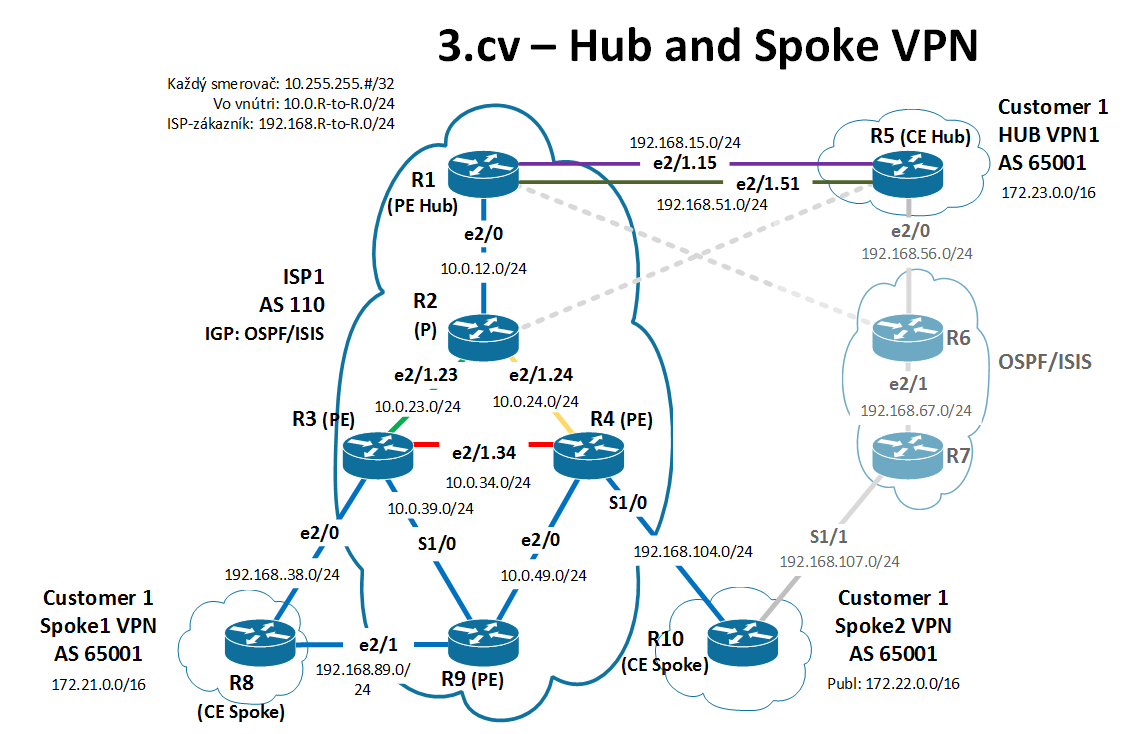
\includegraphics[width=14cm,keepaspectratio]{mpls_hub_spoke_topo}
\caption{Topológia MPLS Hub \& Spoke}
\label{fig:mpls_hub_spoke_topo}
\end{figure}

\begin{figure}[!htbp]
\centering
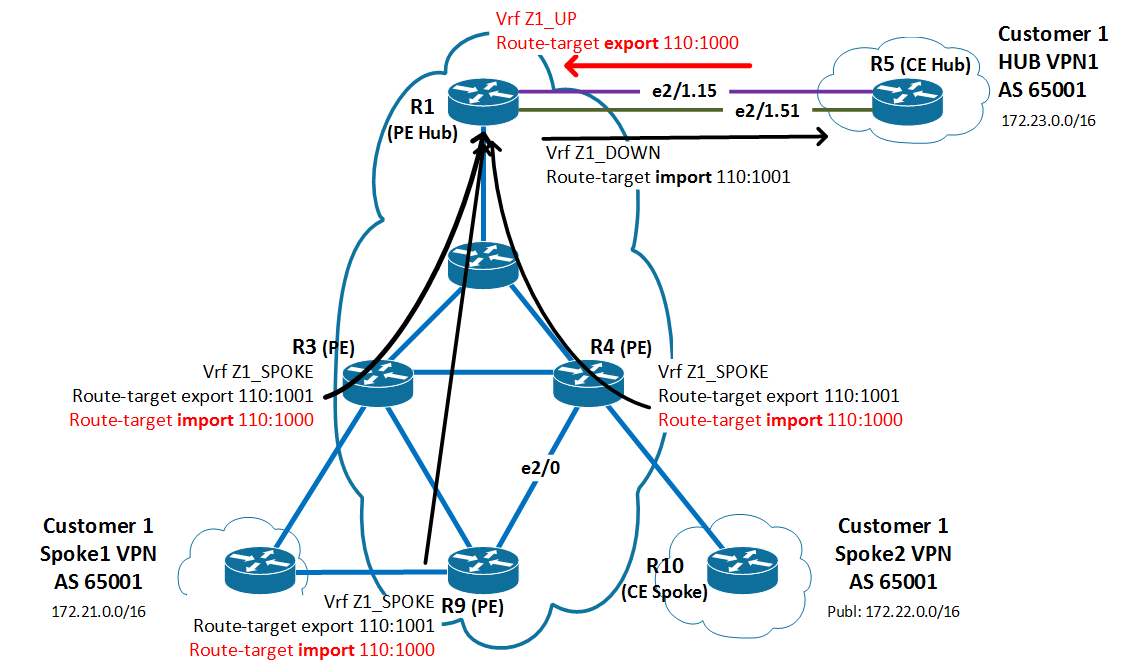
\includegraphics[width=14cm,keepaspectratio]{mpls_hub_spoke_route_target_topo}
\caption{Topológia MPLS Hub \& Spoke s Route Target}
\label{fig:mpls_hub_spoke_route_target_topo}
\end{figure}

\subsubsection{Konfigurácia}
\paragraph{}

\noindent
{\fontfamily{qcr}\selectfont
\begin{small}
\begin{alltt}
R5 (CE smerovač)
router bgp 65001
  address-family ipv4 unicast
    network 10.255.255.5 mask 255.255.255.255
    network 172.23.0.0 mask 255.255.255.0
    neighbor 192.168.15.1 activate
\end{alltt}
\end{small}
}

\paragraph{}
Pokračovali sme konfiguráciou 

\noindent
{\fontfamily{qcr}\selectfont
\begin{small}
\begin{alltt}
R1
no ip vrf RED

ip vrf Z1_DOWN
 rd 110:1001
 route-target import 110:1001

ip vrf Z1_UP
 rd 110:1000
 route-target export 110:1000

interface Ethernet2/1
 no ip address
 duplex half

interface Ethernet2/1.15
 encapsulation dot1Q 15
 ip vrf forwarding Z1_UP
 ip address 192.168.15.1 255.255.255.0

interface Ethernet2/1.51
 encapsulation dot1Q 51
 ip vrf forwarding Z1_DOWN
 ip address 192.168.51.1 255.255.255.0

router bgp 110
 address-family ipv4
  neighbor 10.255.255.3 activate
  neighbor 10.255.255.4 activate
  neighbor 10.255.255.9 activate
 exit-address-family
 
 address-family ipv4 vrf Z1_DOWN
  redistribute connected
  neighbor 192.168.51.5 remote-as 65001
  neighbor 192.168.51.5 activate
  neighbor 192.168.51.5 as-override
 exit-address-family
 
 address-family ipv4 vrf Z1_UP
  redistribute connected
  redistribute static
  neighbor 192.168.15.5 remote-as 65001
  neighbor 192.168.15.5 activate
  neighbor 192.168.15.5 as-override
  default-information originate
 exit-address-family

ip route vrf Z1_UP 0.0.0.0 0.0.0.0 192.168.15.5
mpls ldp router-id Loopback0
==============================================
R3#
no ip vrf RED

int eth2/0
 ip addr 192.168.38.3

ip vrf Z1_SPOKE
 rd 110:1001
 route-target export 110:1001
 route-target import 110:1000

interface Ethernet2/0
 ip vrf forwarding Z1_SPOKE

router bgp 110
 address-family ipv4 vrf Z1_SPOKE
  redistribute connected
  neighbor 192.168.38.8 remote-as 65001
  neighbor 192.168.38.8 activate
  neighbor 192.168.38.8 as-override
 exit-address-family
=======================================
R4#sh run
!ip brf GREEN a RED zmazal a dal:

int s1/0
 ip addr 192.168.104.4 255.255.255.0

int e2/0
 ip addr 10.0.49.4 255.255.255.0

ip vrf Z1_SPOKE
 rd 110:1001
 route-target export 110:1001
 route-target import 110:1000

interface Serial1/0
 ip vrf forwarding Z1_SPOKE

router bgp 110
!namiesto RED a GREEN dal:

 address-family ipv4 vrf Z1_SPOKE
  redistribute connected
  neighbor 192.168.104.10 remote-as 65001
  neighbor 192.168.104.10 activate
  neighbor 192.168.104.10 as-override
 exit-address-family
=================================================
R9#
!ip vrf RED zmenil na:

ip vrf Z1_SPOKE
 rd 110:1001
 route-target export 110:1001
 route-target import 110:1000

interface Ethernet2/1
 ip addr 192.168.89.9 255.255.255.0
 ip vrf forwarding Z1_SPOKE

router bgp 110
!namiesto RED dal:

 address-family ipv4 vrf Z1_SPOKE
  redistribute connected
  neighbor 192.168.38.8 remote-as 65001
  neighbor 192.168.38.8 activate
  neighbor 192.168.38.8 as-override
 exit-address-family
============
R5

interface Ethernet2/1
 no ip address

interface Ethernet2/1.15
 encapsulation dot1Q 15
 ip address 192.168.15.5 255.255.255.0

interface Ethernet2/1.51
 encapsulation dot1Q 51
 ip address 192.168.51.5 255.255.255.0

router bgp 65001
 network 10.255.255.5 mask 255.255.255.255
 neighbor 192.168.15.1 remote-as 110
 neighbor 192.168.51.1 remote-as 110
\end{alltt}
\end{small}
}

\paragraph{}
Parameter as-override zabezpečí, aby smerovače nezahadzovali siete, ktoré prechádzajú do rovnakého AS (65001). Príkaz redistribute connected distribuuje všetky pripojené siete zákazníka v rámci BGP. Tieto príkazy zadáme na smerovačoch R1 smerom k R5, na R9 k R8 a na R4 k R10.

\paragraph{}
Konfigurácia CE smerovačov je podobná, využíva však address-family, pretože zákazníci sa o VRF nezaujímajú. Na smerovačoch R5, R8 a R10 musíme zmeniť predošlú konfiguráciu BGP, teda pôvodné AS nahradíme AS 65001, ohlásime ich vlastné siete a aktivujeme spojenie na suseda.

\noindent
{\fontfamily{qcr}\selectfont
\begin{small}
\begin{alltt}
R5 (CE smerovač)
router bgp 65001
  address-family ipv4 unicast
    network 10.255.255.5 mask 255.255.255.255
    network 172.23.0.0 mask 255.255.255.0
    neighbor 192.168.15.1 activate
\end{alltt}
\end{small}
}

\subsubsection{Overenie}
\paragraph{}
Zadaním tohto príkazu sa presunie záznam z globálnej smerovacej tabuľky do smerovacej tabuľky vrf z1. Po zadaní príkazu je takisto potrebné na ňom nanovo zadať IP adresu. Overenie, že sa rozhranie pridalo do danej VRF, vykonáme príkazom \say{sh ip vrf}.

\noindent
{\fontfamily{qcr}\selectfont
\begin{small}
\begin{alltt}
R1#show ip vrf
  Name                             Default RD          Interfaces  
  Z1_DOWN                               110:2            Et2/1.15
  Z1_UP                                 110:2            Et2/1.51
\end{alltt}
\end{small}
}

\paragraph{}
Po správnej konfigurácii by sa na CE smerovačoch v BGP tabuľke pre ipv4 unicast mali objaviť všetky ohlasované siete smerovačov R5, R8 a R10 (Lo0 aj Lo1).

\noindent
{\fontfamily{qcr}\selectfont
\begin{small}
\begin{alltt}
R8#
...
     Network          Next Hop            Metric LocPrf Weight Path
 *   10.255.255.5/32  192.168.89.9                           0 110 110 i
 *>                   192.168.38.3                           0 110 110 i
 *>  10.255.255.8/32  0.0.0.0                  0         32768 i
 *   10.255.255.10/32 192.168.89.9                           0 110 110 i
 *>                   192.168.38.3                           0 110 110 i
 *>  172.21.0.0       0.0.0.0                  0         32768 ?
 *   172.22.0.0       192.168.89.9                           0 110 110 ?
 *>                   192.168.38.3                           0 110 110 ?
 *   172.23.0.0       192.168.89.9                           0 110 110 ?
 *>                   192.168.38.3                           0 110 110 ?
...
\end{alltt}
\end{small}
}

\paragraph{}
Rovnako sme použili traceroute z R8 (lo1) na R10 (lo1):

\noindent
{\fontfamily{qcr}\selectfont
\begin{small}
\begin{alltt}
R8#traceroute 172.22.0.1 source lo0       
Type escape sequence to abort.
Tracing the route to 172.22.0.1
VRF info: (vrf in name/id, vrf out name/id)
  1 192.168.38.3 16 msec 52 msec 16 msec
  2 192.168.15.1 [AS 110] [MPLS: Label 34 Exp 0] 13 msec 19 msec 66 msec
  3 192.168.51.1 [AS 110] [MPLS: Label 21 Exp 0] 16 msec 20 msec 60 msec
  4 192.168.104.4 [AS 110] [MPLS: Label 29 Exp 0] 18 msec 25 msec 40 msec
  5 192.168.104.10 [AS 110] 60 msec *  72 msec
\end{alltt}
\end{small}
}

\paragraph{}
Z výpisu \say{show ip vrf} vyplýva, že obidve subrozhrania medzi R1 a R5 (pre odoslanú a prijatú premávku) patria do VRF s názvom Z1\_SPOKE. Výpis príkazu \say{sh ip bgp ipv4 unicast} ukazuje naučené lo0 a lo1 rozhrania od R5, R8 a R10. Nakoniec vo výpise príkazu traceroute z R8 na R10 vidíme, že premávka smeruje zo spoke smerovača najprv na hub R5 a odtiaľ späť na spoke R10.









\subsection{Draft Rosen}
\subsubsection{Popis}
\paragraph{}
Draft Rosen je multicastová MPLS technológia pre VPN, ktorá na riadenie multicastovej premávky používa BGP. Topológiu môžeme vidieť na obr. \ref{fig:mpls_l3vpn_draft_rosen_topo}.

\begin{figure}[!htbp]
\centering
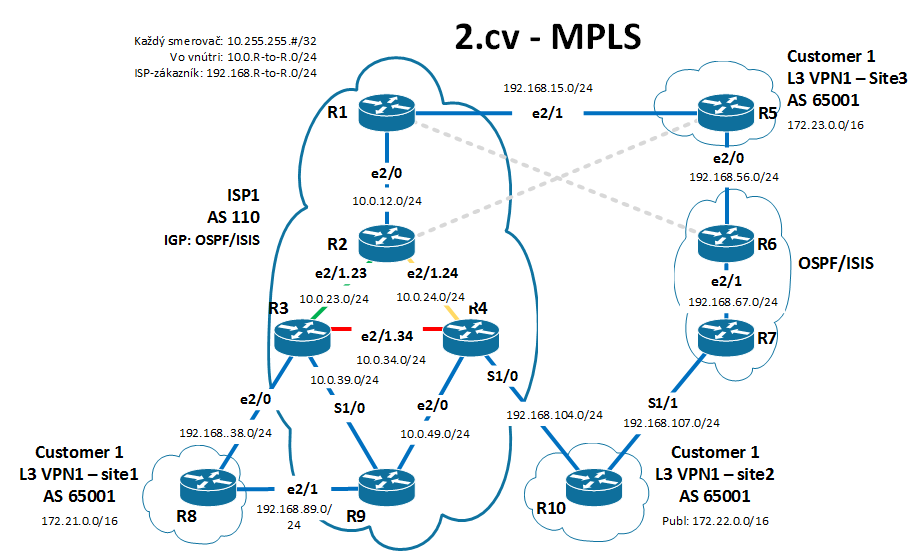
\includegraphics[width=14cm,keepaspectratio]{mpls_l3vpn_topo}
\caption{Topológia Draft Rosen}
\label{fig:mpls_l3vpn_draft_rosen_topo}
\end{figure}

\subsubsection{Konfigurácia}
\paragraph{}
Najprv zrušíme všetko, čo sme nakonfigurovali pri Hub \& Spoke:

\paragraph{}
Zrušíme subrozhrania medzi R1 a R5 a urobíme medzi nimi iba jednu linku.
\noindent
{\fontfamily{qcr}\selectfont
\begin{small}
\begin{alltt}
no int eth2/1.15
no int eth2/1.51
int eth2/1
ip addr 192.168.15.# 255.255.255.0
\end{alltt}
\end{small}
}

Vymažeme IPčku druhého spätného subinterfejsu eth2/1.51 \say{192.168.51.1} z neighbrov v BGP na R5.

\noindent
{\fontfamily{qcr}\selectfont
\begin{small}
\begin{alltt}
R5(config)#router bgp 65001
  no neighbor 192.168.51.1 remote-as 110
\end{alltt}
\end{small}
}


\paragraph{}
Vymažeme VRF z Hub \& Spoke.

\noindent
{\fontfamily{qcr}\selectfont
\begin{small}
\begin{alltt}
!R1
no ip vrf Z1_DOWN
no ip vrf Z1_UP

!R3, R4, R9
no ip vrf Z1_SPOKE
\end{alltt}
\end{small}
}

\paragraph{}
Vytvoríme novú VRF pre klienta GREEN. Route target import a export pre ne bude rovnaký. Novú VRF nastavíme na R1, R3, R4 a R9.

\noindent
{\fontfamily{qcr}\selectfont
\begin{small}
\begin{alltt}
ip vrf GREEN
  rd 110:2
  route-target both 110:2
\end{alltt}
\end{small}
}

\paragraph{}
VRF GREEN aplikujeme na rozhrania R1, R3, R4 a R9 a nanovo nastavíme IP adresy na na rozhraniach, pretože tým, že sme zrušili pôvodné VRF, odstránili sa zároveň IP adresy z rozhraní, na ktorých boli nastavené.

\noindent
{\fontfamily{qcr}\selectfont
\begin{small}
\begin{alltt}
!R1
R1(config)#int eth2/1
R1(config-if)#ip vrf forwarding GREEN
% Interface Ethernet2/1 IPv4 disabled and address(es) removed due to enabling VRF GREEN
R1(config-if)#ip addr 192.168.15.1 255.255.255.0
R1(config-if)#no shut
R1(config-if)#exit
R1(config)#router bgp 110          
R1(config-router)#address-family ipv4 vrf GREEN
R1(config-router-af)#redistribute connected
R1(config-router-af)#neighbor 192.168.15.5 remote-as 65001
R1(config-router-af)#neighbor 192.168.15.5 activa         
*May 16 10:10:08.158: %BGP-5-ADJCHANGE: neighbor 192.168.15.5 vpn vrf GREEN Up 
R1(config-router-af)#neighbor 192.168.15.5 activate
R1(config-router-af)#neighbor 192.168.15.5 as-ov   
R1(config-router-af)#neighbor 192.168.15.5 as-override
\end{alltt}
\end{small}
}

Teraz môžeme začať konfigurovať Draft Rosen. IP adresa multicastovej skupiny (MDT ID) pre zákaznika GREEN je 239.10.10.10. V sieti zákaznika je potrebné nastaviť PIM sparse mode. RP bude R1, v sieti zakaznika to bude R5. konfigurujeme zákaznicke routre R5, R8 a R10. Zákaznícke smerovače potom staticky pripojíme do multicastovej skupiny a overíme funkčnosť.

\paragraph{}
Na všetkých smerovačoch zadáme nižšie uvedený príkaz, aby sme aktivovali multicastové smerovanie.
\noindent
{\fontfamily{qcr}\selectfont
\begin{small}
\begin{alltt}
ip multicast-routing
\end{alltt}
\end{small}
}


\paragraph{}
Na PE smerovačoch (R1, R3, R4, R9) aktivujeme multicastové smerovanie aj pre VRF GREEN.

\noindent
{\fontfamily{qcr}\selectfont
\begin{small}
\begin{alltt}
ip multicast-routing vrf GREEN
\end{alltt}
\end{small}
}



\paragraph{}
Na všetkých providerských smerovačoch zadáme pre všetky rozhrania, ktoré sa podieľajú na multicastovom prenose (aj na loopback0), príkaz:

\noindent
{\fontfamily{qcr}\selectfont
\begin{small}
\begin{alltt}
ip pim sparse-mode
\end{alltt}
\end{small}
}

\paragraph{}
Tým aktivujeme PIM Sparse Mode, ktorý bude prenášať dátový multicastový tok. V trojuholníku stačí dávať príkaz iba na subrozhrania. Tento príkaz vykonáme aj na CE routroch, ale iba pre rozhrania smerujúce ku PE smerovačom.

\paragraph{}
Nastavíme RP pre providera na R1 a pre zakaznika na R5.

\paragraph{}
PE smerovače:
\noindent
{\fontfamily{qcr}\selectfont
\begin{small}
\begin{alltt}
R3(config)#ip pim rp-address 10.255.255.1
\end{alltt}
\end{small}
}

\paragraph{}
Zákaznicke CE smerovače:
\noindent
{\fontfamily{qcr}\selectfont
\begin{small}
\begin{alltt}
R8(config)#ip pim rp-address 172.23.0.1
\end{alltt}
\end{small}
}


\paragraph{}
PE smerovače priradíme do multicastovej skupiny.

\noindent
{\fontfamily{qcr}\selectfont
\begin{small}
\begin{alltt}
R1(config)#ip vrf GREEN
  mdt default 239.10.10.10
\end{alltt}
\end{small}
}

\paragraph{}
Na PE smerovačoch nastavíme zákaznicky RP pre VRF GREEN na R5.

\noindent
{\fontfamily{qcr}\selectfont
\begin{small}
\begin{alltt}
R9(config)#ip pim vrf GREEN rp-address 172.23.0.1
\end{alltt}
\end{small}
}


\paragraph{}
Na CE smerovačoch priradíme loopback1 do multicastovej skupiny

\noindent
{\fontfamily{qcr}\selectfont
\begin{small}
\begin{alltt}
int lo1
  ip igmp join-group 239.10.10.10
\end{alltt}
\end{small}
}





\subsubsection{Overenie MP-BGP konektivity}
\paragraph{}
Najprv sme overovali základnú MP−BGP konektivitu príkazmi \say{sh ip route vrf GREEN} z R4, \say{show ip bgp ipv4 unicast} z R8, \say{ping 172.22.0.1 source 172.21.0.1} z R8 a \say{ping vrf GREEN 172.23.0.1} z R4.

\noindent
{\fontfamily{qcr}\selectfont
\begin{small}
\begin{alltt}
R4(config-router-af)#do sh ip route vrf GREEN

Routing Table: GREEN
...

Gateway of last resort is not set

      10.0.0.0/32 is subnetted, 3 subnets
B        10.255.255.5 [200/0] via 10.255.255.1, 00:08:23
B        10.255.255.8 [200/0] via 10.255.255.3, 00:03:21
B        10.255.255.10 [20/0] via 192.168.104.10, 00:00:23
B     172.21.0.0/16 [200/0] via 10.255.255.3, 00:03:21
B     172.22.0.0/16 [20/0] via 192.168.104.10, 00:00:23
B     172.23.0.0/16 [200/0] via 10.255.255.1, 00:08:23
B     192.168.15.0/24 [200/0] via 10.255.255.1, 00:08:53
B     192.168.38.0/24 [200/0] via 10.255.255.3, 00:04:05
B     192.168.56.0/24 [200/0] via 10.255.255.1, 00:08:23
B     192.168.89.0/24 [200/0] via 10.255.255.3, 00:03:21
      192.168.104.0/24 is variably subnetted, 2 subnets, 2 masks
C        192.168.104.0/24 is directly connected, Serial1/0
L        192.168.104.4/32 is directly connected, Serial1/0
B     192.168.107.0/24 [20/0] via 192.168.104.10, 00:00:23





R8#show ip bgp ipv4 unicast 
BGP table version is 42, local router ID is 10.255.255.8
Status codes: s suppressed, d damped, h history, * valid, > best, i - internal, 
              r RIB-failure, S Stale, m multipath, b backup-path, f RT-Filter, 
              x best-external, a additional-path, c RIB-compressed, 
Origin codes: i - IGP, e - EGP, ? - incomplete
RPKI validation codes: V valid, I invalid, N Not found

     Network          Next Hop            Metric LocPrf Weight Path
 *   10.255.255.5/32  192.168.89.9                           0 110 110 i
 *>                   192.168.38.3                           0 110 110 i
 *>  10.255.255.8/32  0.0.0.0                  0         32768 ?
 *   10.255.255.10/32 192.168.89.9                           0 110 110 ?
 *>                   192.168.38.3                           0 110 110 ?
 *>  172.21.0.0       0.0.0.0                  0         32768 i
 *   172.22.0.0       192.168.89.9                           0 110 110 i
 *>                   192.168.38.3                           0 110 110 i
 *   172.23.0.0       192.168.89.9                           0 110 110 i
 *>                   192.168.38.3                           0 110 110 i
 *   192.168.15.0     192.168.89.9                           0 110 ?
 *>                   192.168.38.3                           0 110 ?
 *   192.168.38.0     192.168.89.9                           0 110 ?
 *                    192.168.38.3             0             0 110 ?
     Network          Next Hop            Metric LocPrf Weight Path
 *>                   0.0.0.0                  0         32768 ?
 *   192.168.56.0     192.168.89.9                           0 110 110 ?
 *>                   192.168.38.3                           0 110 110 ?
 *   192.168.89.0     192.168.89.9             0             0 110 ?
 *                    192.168.38.3                           0 110 ?
 *>                   0.0.0.0                  0         32768 ?
 *   192.168.104.0    192.168.89.9                           0 110 ?
 *>                   192.168.38.3                           0 110 ?
 *   192.168.107.0    192.168.89.9                           0 110 110 ?
 *>                   192.168.38.3                           0 110 110 ?







R8#ping 172.22.0.1 source 172.21.0.1
Type escape sequence to abort.
Sending 5, 100-byte ICMP Echos to 172.22.0.1, timeout is 2 seconds:
Packet sent with a source address of 172.21.0.1 
!!!!!
Success rate is 100 percent (5/5), round-trip min/avg/max = 52/56/60 ms





R4(config-router-af)#do ping vrf GREEN 172.23.0.1
Type escape sequence to abort.
Sending 5, 100-byte ICMP Echos to 172.23.0.1, timeout is 2 seconds:
!!!!!
Success rate is 100 percent (5/5), round-trip min/avg/max = 52/59/72 ms

\end{alltt}
\end{small}
}

\paragraph{}
Z výpisov uvedených vyššie vyplýva, že privátne siete 172.2X.0.0 sa rozšírili medzi všetky PE aj CE smerovače. Výpisy príkazu \say{ping} ukazujú vzájomnú konektivitu medzi pobočkami zákazníka GREEN.

\subsubsection{Overenie Draft Rosen a multicastových tunelov}
\paragraph{}
Draft Rosen sme overovali príkazmi \say{ip pim rp-address 10.255.255.1} z R1 a \say{ping 239.10.10.10 repeat 2} z R5.

\noindent
{\fontfamily{qcr}\selectfont
\begin{small}
\begin{alltt}
R1(config)#ip pim rp-address 10.255.255.1
R1(config)#
*May 16 10:59:35.306: %LINEPROTO-5-UPDOWN: Line protocol on Interface Tunnel0, changed state to up
*May 16 10:59:35.474: %LINEPROTO-5-UPDOWN: Line protocol on Interface Tunnel1, changed state to up

\end{alltt}
\end{small}
}

\noindent
{\fontfamily{qcr}\selectfont
\begin{small}
\begin{alltt}
R5#ping 239.10.10.10 repeat 2 
Type escape sequence to abort.
Sending 2, 100-byte ICMP Echos to 239.10.10.10, timeout is 2 seconds:

Reply to request 0 from 172.23.0.1, 32 ms
Reply to request 0 from 172.21.0.1, 84 ms
Reply to request 0 from 172.22.0.1, 80 ms
Reply to request 1 from 172.23.0.1, 8 ms
Reply to request 1 from 172.21.0.1, 80 ms
Reply to request 1 from 172.22.0.1, 80 ms
\end{alltt}
\end{small}
}

\paragraph{}
Po vykonaní príkazu \say{ip pim rp-address 10.255.255.1} sa zobrazili správy, ktoré hovoria o vytvorení tunelových rozhraní ku smerovačom, ktoré sa nachádzajú v multicastovej doméne. Na ping zákazníckej multicastovej skupiny odpovedali všetky smerovače nachádzajúce sa v zákazníckej multicastovej doméne t.j. R5, R8 a R10.


\end{document}